\documentclass{article}
\usepackage{tikz-qtree}
\begin{document}
\tikzset{every tree node/.style={minimum width=2em,draw,circle},
	    blank/.style={draw=none},
	    edge from parent/.style=
	    {draw,edge from parent path={(\tikzparentnode) -- (\tikzchildnode)}},
	    level distance=1.5cm}
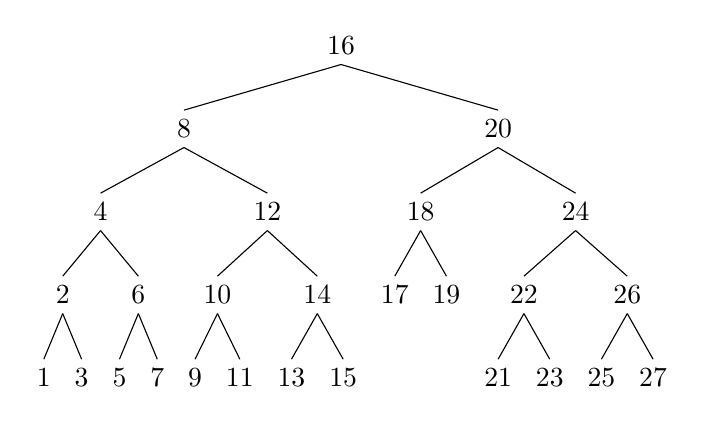
\begin{tikzpicture}
\Tree
[.16
[.8
[.4
[.2
{1}
{3}
]
[.6
{5}
{7}
]
]
[.12
[.10
{9}
{11}
]
[.14
{13}
{15}
]
]
]
[.20
[.18
{17}
{19}
]
[.24
[.22
{21}
{23}
]
[.26
{25}
{27}
]
]
]
]
\end{tikzpicture}
\end{document}
